%╔════════════════════════════╗
%║	  Szablon dostosował	  ║
%║	mgr inż. Dawid Kotlarski  ║
%║		  06.10.2024		  ║
%╚════════════════════════════╝
\documentclass[12pt,twoside,a4paper,openany]{article}

    % ------------------------------------------------------------------------
% PAKIETY
% ------------------------------------------------------------------------

%różne pakiety matematyczne, warto przejrzeć dokumentację, muszą być powyżej ustawień językowych.
\usepackage{mathrsfs}   %Różne symbole matematyczne opisane w katalogu ~\doc\latex\comprehensive. Zamienia \mathcal{L} ze zwykłego L na L-transformatę.
\usepackage{eucal}      %Różne symbole matematyczne.
\usepackage{amssymb}    %Różne symbole matematyczne.
\usepackage{amsmath}    %Dodatkowe funkcje matematyczne, np. polecenie \dfac{}{} skladajace ulamek w trybie wystawionym (porównaj $\dfrac{1}{2}$, a $\frac{1}{2}$).

%język polski i klawiatura
\usepackage[polish]{babel}
\usepackage{csquotes}
%\usepackage{qtimes} % czcionka Times new Roman
\usepackage{polski}

\usepackage{ifluatex}

\ifluatex
  %czcionka
  \usepackage{fontspec}
  \setmainfont{Calibri}

  %obsługa pdf'a
  \usepackage[luatex,usenames,dvipsnames]{color}      %Obsługa kolorów. Opcje usenames i dvipsnames wprowadzają dodatkowe nazwy kolorow.
  \usepackage[luatex,pagebackref=false,draft=false,pdfpagelabels=false,colorlinks=true,urlcolor=cyan,linkcolor=blue,filecolor=magenta,citecolor=green,pdfstartview=FitH,pdfstartpage=1,pdfpagemode=UseOutlines,bookmarks=true,bookmarksopen=true,bookmarksopenlevel=2,bookmarksnumbered=true,pdfauthor={Dawid Kotlarski},pdftitle={Dokumentacja Projektowa},pdfsubject={},pdfkeywords={transient recovery voltage trv},unicode=true]{hyperref}   %Opcja pagebackref=true dotyczy bibliografii: pokazuje w spisie literatury numery stron, na których odwołano się do danej pozycji.
\else
  \usepackage[pdftex,usenames,dvipsnames]{color}      %Obsługa kolorów. Opcje usenames i dvipsnames wprowadzają dodatkowe nazwy kolorow.
  \usepackage[pdftex,pagebackref=false,draft=false,pdfpagelabels=false,colorlinks=true,urlcolor=cyan,linkcolor=blue,filecolor=magenta,citecolor=green,pdfstartview=FitH,pdfstartpage=1,pdfpagemode=UseOutlines,bookmarks=true,bookmarksopen=true,bookmarksopenlevel=2,bookmarksnumbered=true,pdfauthor={Dawid Kotlarski},pdftitle={Dokumentacja Projektowa},pdfsubject={},pdfkeywords={transient recovery voltage trv},unicode=true]{hyperref}   %Opcja pagebackref=true dotyczy bibliografii: pokazuje w spisie literatury numery stron, na których odwołano się do danej pozycji.
\fi

%bibliografia
%\usepackage[numbers,sort&compress]{natbib}  %Porządkuje zawartość odnośników do literatury, np. [2-4,6]. Musi być pod pdf'em, a styl bibliogfafii musi mieć nazwę z dodatkiem 'nat', np. \bibliographystyle{unsrtnat} (w kolejności cytowania).
\usepackage[
  backend=biber,
  style=numeric,
  sorting=none
]{biblatex}
\addbibresource{bibliografia.bib}
\usepackage{hypernat}                       %Potrzebna pakietowi natbib do wspolpracy z pakietem hyperref (wazna kolejnosc: 1. hyperref, 2. natbib, 3. hypernat).

%grafika i geometria strony
\usepackage{extsizes}           %Dostepne inne rozmiary czcionek, np. 14 w poleceniu: \documentclass[14pt]{article}.
\usepackage[final]{graphicx}
\usepackage[a4paper,left=3.5cm,right=2.5cm,top=2.5cm,bottom=2.5cm]{geometry}

%strona tytułowa
\usepackage{strona_tytulowa}

%inne
\usepackage{lastpage} %! do numerowania stron w formacie (x z y)
\usepackage[hide]{todo}                     %Wprowadza polecenie \todo{treść}. Opcje pakietu: hide/show. Polecenie \todos ma byc na koncu dokumentu, wszystkie \todo{} po \todos sa ignorowane.
\usepackage[basic,physics]{circ}            %Wprowadza środowisko circuit do rysowania obwodów elektrycznych. Musi byc poniżej pakietow językowych.
\usepackage[sf,bf,outermarks]{titlesec}     %Troszczy się o wygląd tytułów rozdziałów (section, subsection, ...). sf oznacza czcionkę sans serif (typu arial), bf -- bold. U mnie: oddzielna linia dla naglowku paragraph. Patrz tez: tocloft -- lepiej robi format spisu tresci.
\usepackage{tocloft}                        %Troszczy się o format spisu trsci.
\usepackage{expdlist}    %Zmienia definicję środowiska description, daje większe możliwości wpływu na wygląd listy.
\usepackage{flafter}     %Wprowadza parametr [tb] do polecenia \suppressfloats[t] (polecenie to powoduje nie umieszczanie rysunkow, tabel itp. na stronach, na ktorych jest to polecenie (np. moze byc to stroma z tytulem rozdzialu, ktory chcemy zeby byl u samej gory, a nie np. pod rysunkiem)).
\usepackage{array}       %Ładniej drukuje tabelki (np. daje wiecej miejsca w komorkach -- nie są tak ścieśnione, jak bez tego pakietu).
\usepackage{listings}    %Listingi programow.
\usepackage[format=hang,labelsep=period,labelfont={bf,small},textfont=small]{caption}   %Formatuje podpisy pod rysunkami i tabelami. Parametr 'hang' powoduje wcięcie kolejnych linii podpisu na szerokosc nazwy podpisu, np. 'Rysunek 1.'.
\usepackage{appendix}    %Troszczy się o załączniki.
\usepackage{floatflt}    %Troszczy się o oblewanie rysunkow tekstem.
\usepackage{here}        %Wprowadza dodtkowy parametr umiejscowienia rysunków, tabel, itp.: H (duże). Umiejscawia obiekty ruchome dokladnie tam gdzie są w kodzie źródłowym dokumentu.
\usepackage{makeidx}     %Troszczy się o indeks (skorowidz).

%nieużywane, ale potencjalnie przydatne
\usepackage{sectsty}           %Formatuje nagłówki, np. żeby były kolorowe -- polecenie: \allsectionsfont{\color{Blue}}.
%\usepackage{version}           %Wersje dokumentu.

%============
\usepackage{longtable}			%tabelka
%============

%============
% Ustawienia listingów do kodu
%============

\usepackage{listings}
\usepackage{xcolor}

\definecolor{codegreen}{rgb}{0,0.6,0}
\definecolor{codegray}{rgb}{0.5,0.5,0.5}
\definecolor{codepurple}{rgb}{0.58,0,0.82}
\definecolor{backcolour}{rgb}{0.95,0.95,0.92}

% Definicja stylu "mystyle"
\lstdefinestyle{mystyle}{
backgroundcolor=\color{backcolour},
commentstyle=\color{codegreen},
keywordstyle=\color{blue},	%magenta
numberstyle=\tiny\color{codegray},
stringstyle=\color{codepurple},
basicstyle=\ttfamily\footnotesize,
breakatwhitespace=false,
breaklines=true,
captionpos=b,
keepspaces=true,
numbers=left,
numbersep=5pt,
showspaces=false,
showstringspaces=false,
showtabs=false,
tabsize=2,
literate=
  {á}{{\'a}}1 {é}{{\'e}}1 {í}{{\'i}}1 {ó}{{\'o}}1 {ú}{{\'u}}1
{Á}{{\'A}}1 {É}{{\'E}}1 {Í}{{\'I}}1 {Ó}{{\'O}}1 {Ú}{{\'U}}1
{à}{{\`a}}1 {è}{{\`e}}1 {ì}{{\`i}}1 {ò}{{\`o}}1 {ù}{{\`u}}1
{À}{{\`A}}1 {È}{{\`E}}1 {Ì}{{\`I}}1 {Ò}{{\`O}}1 {Ù}{{\`U}}1
{ä}{{\"a}}1 {ë}{{\"e}}1 {ï}{{\"i}}1 {ö}{{\"o}}1 {ü}{{\"u}}1
{Ä}{{\"A}}1 {Ë}{{\"E}}1 {Ï}{{\"I}}1 {Ö}{{\"O}}1 {Ü}{{\"U}}1
{â}{{\^a}}1 {ê}{{\^e}}1 {î}{{\^i}}1 {ô}{{\^o}}1 {û}{{\^u}}1
{Â}{{\^A}}1 {Ê}{{\^E}}1 {Î}{{\^I}}1 {Ô}{{\^O}}1 {Û}{{\^U}}1
{ã}{{\~a}}1 {ẽ}{{\~e}}1 {ĩ}{{\~i}}1 {õ}{{\~o}}1 {ũ}{{\~u}}1
{Ã}{{\~A}}1 {Ẽ}{{\~E}}1 {Ĩ}{{\~I}}1 {Õ}{{\~O}}1 {Ũ}{{\~U}}1
{œ}{{\oe}}1 {Œ}{{\OE}}1 {æ}{{\ae}}1 {Æ}{{\AE}}1 {ß}{{\ss}}1
{ű}{{\H{u}}}1 {Ű}{{\H{U}}}1 {ő}{{\H{o}}}1 {Ő}{{\H{O}}}1
{ç}{{\c c}}1 {Ç}{{\c C}}1 {ø}{{\o}}1 {Ø}{{\O}}1 {å}{{\r a}}1 {Å}{{\r A}}1
{€}{{\euro}}1 {£}{{\pounds}}1 {«}{{\guillemotleft}}1
{»}{{\guillemotright}}1 {ñ}{{\~n}}1 {Ñ}{{\~N}}1 {¿}{{?`}}1 {¡}{{!`}}1
{ą}{{\k{a}}}1 {ć}{{\'{c}}}1 {ę}{{\k{e}}}1 {ł}{{\l}}1 {ń}{{\'n}}1
{ó}{{\'o}}1 {ś}{{\'s}}1 {ź}{{\'z}}1 {ż}{{\.{z}}}1
{Ą}{{\k{A}}}1 {Ć}{{\'{C}}}1 {Ę}{{\k{E}}}1 {Ł}{{\L}}1 {Ń}{{\'N}}1
{Ó}{{\'O}}1 {Ś}{{\'S}}1 {Ź}{{\'Z}}1 {Ż}{{\.{Z}}}1
}

\lstset{style=mystyle} % Deklaracja aktywnego stylu
%===========

%PAGINA GÓRNA I DOLNA
\usepackage{fancyhdr}          %Dodaje naglowki jakie się chce.
\pagestyle{fancy}
\fancyhf{}
% numery stron w paginie dolnej na srodku
\fancyfoot[C]{\footnotesize DOKUMENTACJA PROJEKTU – SYSTEMY OPERACYJNE  \\
  \normalsize\sffamily  \thepage\ z~\pageref{LastPage}}


%\fancyhead[L]{\small\sffamily \nouppercase{\leftmark}}
\fancyhead[C]{\footnotesize \textit{AKADEMIA NAUK STOSOWANYCH W NOWYM SĄCZU}\\}

\renewcommand{\headrulewidth}{0.4pt}
\renewcommand{\footrulewidth}{0.4pt}

    % ------------------------------------------------------------------------
% USTAWIENIA
% ------------------------------------------------------------------------

% ------------------------------------------------------------------------
%   Kropki po numerach sekcji, podsekcji, itd.
%   Np. 1.2. Tytuł podrozdziału
% ------------------------------------------------------------------------
\makeatletter
    \def\numberline#1{\hb@xt@\@tempdima{#1.\hfil}}                      %kropki w spisie treści
    \renewcommand*\@seccntformat[1]{\csname the#1\endcsname.\enspace}   %kropki w treści dokumentu
\makeatother

% ------------------------------------------------------------------------
%   Numeracja równań, rysunków i tabel
%   Np.: (1.2), gdzie:
%   1 - numer sekcji, 2 - numer równania, rysunku, tabeli
%   Uwaga ogólna: o otoczeniu figure ma być najpierw \caption{}, potem \label{}, inaczej odnośnik nie działa!
% ------------------------------------------------------------------------
\makeatletter
    \@addtoreset{equation}{section} %resetuje licznik po rozpoczęciu nowej sekcji
    \renewcommand{\theequation}{{\thesection}.\@arabic\c@equation} %dodaje kropki

    \@addtoreset{figure}{section}
    \renewcommand{\thefigure}{{\thesection}.\@arabic\c@figure}

    \@addtoreset{table}{section}
    \renewcommand{\thetable}{{\thesection}.\@arabic\c@table}
\makeatother

% ------------------------------------------------------------------------
% Tablica
% ------------------------------------------------------------------------
\newenvironment{tabela}[3]
{
    \begin{table}[!htb]
    \centering
    \caption[#1]{#2}
    \vskip 9pt
    #3
}{
    \end{table}
}

% ------------------------------------------------------------------------
% Dostosowanie wyglądu pozycji listy \todos, np. zamiast 'p.' jest 'str.'
% ------------------------------------------------------------------------
\renewcommand{\todoitem}[2]{%
    \item \label{todo:\thetodo}%
    \ifx#1\todomark%
        \else\textbf{#1 }%
    \fi%
    (str.~\pageref{todopage:\thetodo})\ #2}
\renewcommand{\todoname}{Do zrobienia...}
\renewcommand{\todomark}{~uzupełnić}

% ------------------------------------------------------------------------
% Definicje
% ------------------------------------------------------------------------
\def\nonumsection#1{%
    \section*{#1}%
    \addcontentsline{toc}{section}{#1}%
    }
\def\nonumsubsection#1{%
    \subsection*{#1}%
    \addcontentsline{toc}{subsection}{#1}%
    }
\reversemarginpar %umieszcza notki po lewej stronie, czyli tam gdzie jest więcej miejsca
\def\notka#1{%
    \marginpar{\footnotesize{#1}}%
    }
\def\mathcal#1{%
    \mathscr{#1}%
    }
\newcommand{\atp}{ATP/EMTP} % Inaczej: \def\atp{ATP/EMTP}

% ------------------------------------------------------------------------
% Inne
% ------------------------------------------------------------------------
\frenchspacing                      
\hyphenation{ATP/-EMTP}             %dzielenie wyrazu w danym miejscu
\setlength{\parskip}{3pt}           %odstęp pomiędzy akapitami
\linespread{1.3}                    %odstęp pomiędzy liniami (interlinia)
\setcounter{tocdepth}{4}            %uwzględnianie w spisie treści czterech poziomów sekcji
\setcounter{secnumdepth}{4}         %numerowanie do czwartego poziomu sekcji 
\titleformat{\paragraph}[hang]      %wygląd nagłówków
{\normalfont\sffamily\bfseries}{\theparagraph}{1em}{}

%komenda do łatwiejszego wstawiania zdjęć
\newcommand*{\fg}[4][\textwidth]{
    \begin{figure}[!htb]
        \begin{center}
            \includegraphics[width=#1]{#2}
            \caption{#3}
            \label{rys:#4}
        \end{center}
    \end{figure}
}

\newcommand*{\Oznacz}[2]{
\ref{#1:#2} (s. \pageref{#1:#2})
}

\newcommand*{\OznaczZdjecie}[2][Rysunek]{
#1 \Oznacz{rys}{#2}
}
    
\newcommand*{\OznaczKod}[1]{
\Oznacz{lst}{#1}
}

\newcommand*{\ListingFile}[2]{
    \lstinputlisting[caption=#1, label={lst:#2}, language=C++]{kod/#2.txt}
}


    %polecenia zdefiniowane w pakiecie strona_tytulowa.sty
    \title{...Algorytm listy dwukierunkowej \\z zastosowaniem GitHub...}		%...Wpisać nazwę projektu...
    \author{Imie Nazwisko}
    \authorI{}
    \authorII{}		%jeśli są dwie osoby w projekcie to zostawiamy:    \authorII{}
		
	\uczelnia{AKADEMIA NAUK STOSOWANYCH \\W NOWYM SĄCZU}
    \instytut{Wydział Nauk Inżynieryjnych}
    \kierunek{Katedra Informatyki}
    \praca{DOKUMENTACJA PROJEKTOWA}
    \przedmiot{ZAAWANSOWANE PROGRAMOWANIE}
    \prowadzacy{mgr inż. Dawid Kotlarski}
    \rok{2024}


%definicja składni mikrotik
\usepackage{fancyvrb}
\DefineVerbatimEnvironment{MT}{Verbatim}%
{commandchars=\+\[\],fontsize=\small,formatcom=\color{red},frame=lines,baselinestretch=1,} 
\let\mt\verb 
%zakonczenie definicji składni mikrotik

\usepackage{fancyhdr}    %biblioteka do nagłówka i stopki

			
\begin{document}
   
    \renewcommand{\figurename}{Rys.}    %musi byc pod \begin{document}, bo w~tym miejscu pakiet 'babel' narzuca swoje ustawienia
    \renewcommand{\tablename}{Tab.}     %j.w.
    \thispagestyle{empty}               %na tej stronie: brak numeru
    \stronatytulowa                     %strona tytułowa tworzona przez pakiet strona_tytulowa.tex
 
 \pagestyle{fancy}

    \newpage

    %formatowanie spisu treści i~nagłówków
    \renewcommand{\cftbeforesecskip}{8pt}
    \renewcommand{\cftsecafterpnum}{\vskip 8pt}
    \renewcommand{\cftparskip}{3pt}
    \renewcommand{\cfttoctitlefont}{\Large\bfseries\sffamily}
    \renewcommand{\cftsecfont}{\bfseries\sffamily}
    \renewcommand{\cftsubsecfont}{\sffamily}
    \renewcommand{\cftsubsubsecfont}{\sffamily}
    \renewcommand{\cftparafont}{\sffamily}
    %koniec formatowania spisu treści i nagłówków
     
    \tableofcontents    %spis treści
    \thispagestyle{fancy}
    \newpage

    
    \newpage

    
%%%%%%%%%%%%%%%%%%% treść główna dokumentu %%%%%%%%%%%%%%%%%%%%%%%%%

   	\newpage
\section{Ogólne określenie wymagań}		%1
%Określenie celu pracy, co chcemy uzyskać, jakie przewidujemy wyniki













\hspace{0.60cm}Tutaj może coś być wpisane. 

\subsection{Przykład}  %1.1       

\hspace{0.60cm}Tak zaczynamy pisanie pierwszego akapitu. Jeśli chcemy napisać przypis do bibliografii wykonujemy to w~ten sposób\footnote{Przykład odnośnika do książki\cite{legierski}.}.

%rysunek
	\begin{figure}[!htb]
	\begin{center}
		
\includegraphics[width=8cm]{rys/ans.png}
		\caption{Logo}
		\label{rys:rysunek001}
	\end{center}
\end{figure}

Tutaj może coś być wpisane. \\Tutaj może coś być wpisane\footnote{Przykład odnośnika do strony www\cite{www1}.}. 
Rysunek \ref{rys:rysunek001} (s. \pageref{rys:rysunek001}) pokazuje przykładową ilustrację.

%tabelka
\begin{tabela}
	%uwaga: w nawiasach [] nie może być odnośnika do literatury, jeżeli w dokumencie jest spis rysunków na początku, a spis literatury jest w kolejności cytowania (zmienia to numeracji)
	{Tabelka przykładowa}	%opis w spisie tabel
	{Tabelka przykładowa}	%opis przy tabeli
	{
		\begin{tabular}{|c|c|} \hline
			$U_n$ & $I_{zw}$ \\ \hline
			$kV$  & $\%$      \\ \hline
			7.2 & 100 \\ \hline
		\end{tabular}
	}
	\label{tab:tablica001}
\end{tabela}

% Kod

Listing kodu

\begin{lstlisting}[caption=Przykładowy kod 001, label={lst:listing-cpp}, language=C++]
#include <iostream>
#include <cstdlib>
#include <ctime>
using namespace std;

/*
liczby pseldolosowe
*/

int main(int argc, char** argv) {
	
	int tab[10][10];
	
	for(int i=0;i<10;i++)
	for(int j=0;j<10;j++)
	tab[i][j]=0;
	
	srand(time(NULL));		//generowanie z czasu
	int min=3;
	int max=7;
	for(int i=0;i<10;i++)
	for(int j=0;j<10;j++)		
	tab[i][j]=(rand()%(max-min+1))+min;	
	
	for(int i=0;i<10;i++)
	{
		for(int j=0;j<10;j++)
		cout<<tab[i][j]<<" ";	
		cout<<endl;
	}
	
	return 0;
}
\end{lstlisting}

Tutaj może coś być wpisane. Tutaj może coś być wpisane. Tutaj może coś być wpisane. Tabela \ref{tab:tablica001} (s. \pageref{tab:tablica001}) pokazuje sposoby użycia trybu matematycznego.

Kod \ref{lst:listing-cpp} (s. \pageref{lst:listing-cpp}) przedstawia sposób generowania liczb pseudolosowych. Kod \ref{lst:listing-cpp2} (s. \pageref{lst:listing-cpp2}) przedstawia generowanie pliku HTML.

Alternatywna metoda wklejenia kodu:

\lstinputlisting[caption=Przykładowy kod 002, label={lst:listing-cpp2}, language=C++]{kod/main.cpp}


\subsection{Instalacja}  %1.2

\hspace{0.60cm}Poniżej są opisane kroki potrzebne do instalacji \LaTeX 'a oraz do używania tego szablonu.

 Na początku instalujemy \TeX{}Live\footnote{Instalka na stronie  https://www.tug.org/texlive/acquire-netinstall.html\cite{www2}.}. Ściągamy plik instalacyjny, zajmuje około 25MB. Podczas instalacji można wybrać do zainstalowania różne kolekcje pakietów. Jeśli nie ma problemów z miejscem na dysku to można zainstalować wszystkie, wtedy nie będzie problemu z brakującymi pakietami i błędami. Po wybraniu kolekcji brakujące pliki są pobierane z internetu. Pełna instalacja programu zajmuje około 8GB. Najlepiej zostawić instalację na noc, ponieważ proces zabiera sporo czasu. Warto ustawić komputer tak, aby się nie wyłączył lub nie uśpił. Warto także przed instalacją zablokować antywirusa, ponieważ może blokować niektóre z komponentów.
 
Następnie instalujemy \TeX{}studio\footnote{Plik instalacyjny na stronie  https://www.texstudio.org\cite{www3}.}. Ściągamy plik instalacyjny zajmujący około 120MB. Instalacja przebiega standardowo.

 %rysunek
\begin{figure}[!hbt]
	\begin{center}
		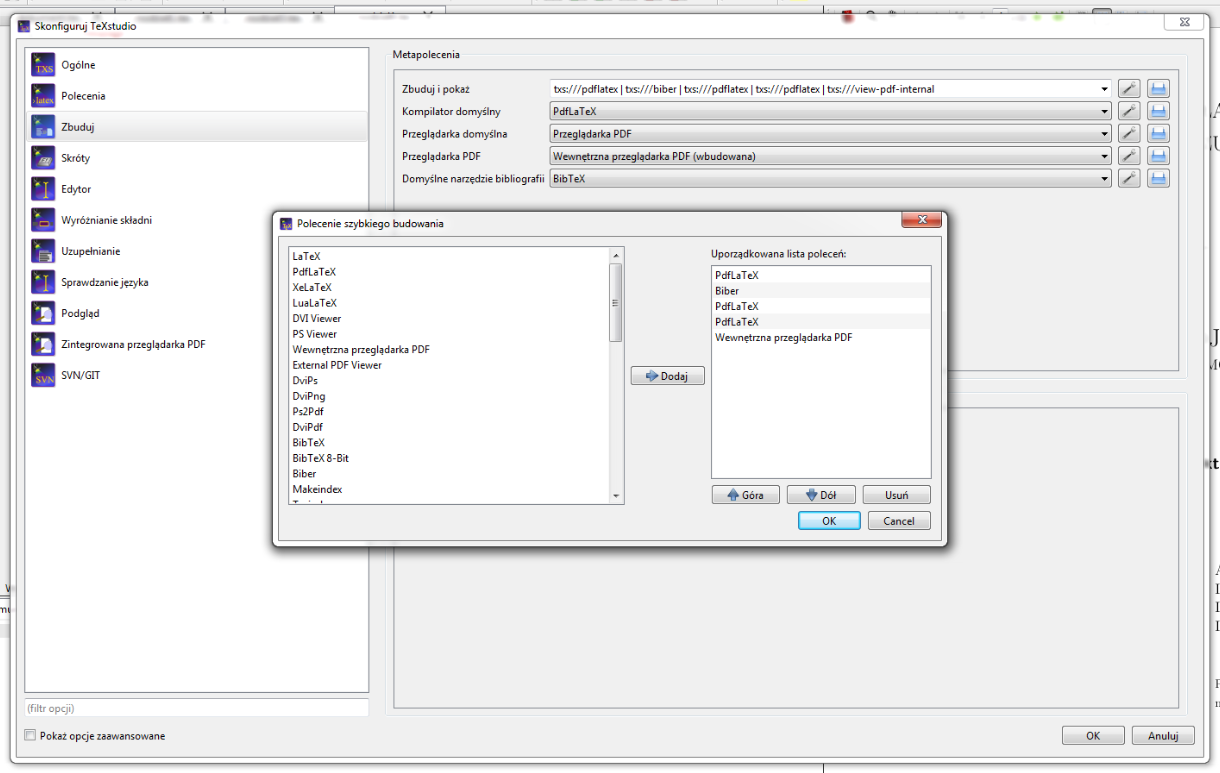
\includegraphics[width=\linewidth]{rys/ustawienie.png}
		\caption{Ustawienie TeXstudio}
		\label{rys:ustawienia}
	\end{center}
\end{figure}

Następnym krokiem jest ustawienie w \TeX{}Studio kolejności budowania projektu. Należy wybrać zakładkę: ,,Opcje/Konfiguruj \TeX{}studio...''. W otwartym oknie przechodzimy na zakładkę ,,Zbuduj''. Na rysunku \ref{rys:ustawienia} (s. \pageref{rys:ustawienia}) pokazany jest zrzut ekranu z konfiguracją. W linijce ,,Zbuduj i pokaż'' klikamy ikonę klucza, żeby przejść do konfiguracji polecenia. W otwartym oknie ustawić kolejność tak jak pokazano na rysunku.

 
 
 
 
 
   \newpage
\section{Analiza problemu}		%2
%Napisać gdzie używa się tego algorytmu
%Opisać sposób działania programu/algorytmu
%Napisać spsoób wykorzystania algorytmu po przez wykonanie przykładu (np. mnożenie macierzy - wykonać ręcznie przykład z mnożeniem macierzy pokazujący jak mnoży się macierz ręcznie)
%Jeśli zadanie zakłada przedstawienie jakiegoś narzędzia (np. git, AI) należy opisać narzędzie




   	\newpage
\section{Projektowanie}		%3
%Napisać z jakich narzędzi będziemy korzystać (kompilator, język programowania), git, biblioteki dodatkowe, itp.
%Opisać szczegółowe ustawienia kompilatora (jeśli są), powiązania z bibliotekami, itp.
%Narysować graf, UML, diagram klas, schemat działania algorytmu
%Jeśli zadanie zakłada przedstawienie jakiegoś narzędzia (np. git, AI) należy opisać sposób jego używania



   	\newpage
\section{Implementacja}		%4
%Opisać implementacje algorytmu/programu. Pokazać ciekawe fragmenty kodu
%Opisać powstałe wyniki (algorytmu/nrzędzia)



   	\newpage
\section{Wnioski}	%5
%Npisać wnioski końcowe z przeprowadzonego projektu, 



   
       
%%%%%%%%%%%%%%%%%%% koniec treść główna dokumentu %%%%%%%%%%%%%%%%%%%%%
	\newpage
    \addcontentsline{toc}{section}{Literatura}  
	\printbibliography

    \newpage
    \hypersetup{linkcolor=black}
    \renewcommand{\cftparskip}{3pt}
    \clearpage
    \renewcommand{\cftloftitlefont}{\Large\bfseries\sffamily}
    \listoffigures
    \addcontentsline{toc}{section}{Spis rysunków}
	\thispagestyle{fancy}
	
    \newpage
    \renewcommand{\cftlottitlefont}{\Large\bfseries\sffamily}
    \def\listtablename{Spis tabel}
    \addcontentsline{toc}{section}{Spis tabel}\listoftables 
	\thispagestyle{fancy}
	
	\newpage
	\renewcommand{\cftlottitlefont}{\Large\bfseries\sffamily}
	\renewcommand\lstlistlistingname{Spis listingów}
	\addcontentsline{toc}{section}{Spis listingów}\lstlistoflistings 
	\thispagestyle{fancy}
	


    %lista rzeczy do zrobienia: wypisuje na koñcu dokumentu, patrz: pakiet todo.sty
    \todos
    %koniec listy rzeczy do zrobienia
\end{document}
